%%%%%%%%%%%%%%%%%%%%%%%%%%%%%%%%%%%%%%%%%
% Jacobs Landscape Poster
% LaTeX Template
% Version 1.1 (14/06/14)
%
% Created by:
% Computational Physics and Biophysics Group, Jacobs University
% https://teamwork.jacobs-university.de:8443/confluence/display/CoPandBiG/LaTeX+Poster
% 
% Further modified by:
% Nathaniel Johnston (nathaniel@njohnston.ca)
%
% This template has been downloaded from:
% http://www.LaTeXTemplates.com
%
% License:
% CC BY-NC-SA 3.0 (http://creativecommons.org/licenses/by-nc-sa/3.0/)
%
%%%%%%%%%%%%%%%%%%%%%%%%%%%%%%%%%%%%%%%%%

%----------------------------------------------------------------------------------------
%	PACKAGES AND OTHER DOCUMENT CONFIGURATIONS
%----------------------------------------------------------------------------------------

\documentclass[final]{beamer}

\usepackage[scale=1.0,width=46.8,height=33.1]{beamerposter} % Use the beamerposter package for laying out the poster
\usetheme{confposter} % Use the confposter theme supplied with this template

\setbeamercolor{block title}{fg=dblue!80,bg=white} % Colors of the block titles
\setbeamercolor{block body}{fg=black,bg=white} % Colors of the body of blocks
\setbeamercolor{block alerted title}{fg=white,bg=dblue!70} % Colors of the highlighted block titles
\setbeamercolor{block alerted body}{fg=black,bg=dblue!10} % Colors of the body of highlighted blocks
% Many more colors are available for use in beamerthemeconfposter.sty

%-----------------------------------------------------------
% Define the column widths and overall poster size
% To set effective sepwid, onecolwid and twocolwid values, first choose how many columns you want and how much separation you want between columns
% In this template, the separation width chosen is 0.024 of the paper width and a 4-column layout
% onecolwid should therefore be (1-(# of columns+1)*sepwid)/# of columns e.g. (1-(4+1)*0.024)/4 = 0.22
% onecolwid should therefore be (1-(# of columns+1)*sepwid)/# of columns e.g. 
% (1-(3+1)*0.025)/3 = 0.3
% Set twocolwid to be (2*onecolwid)+sepwid = 0.464
% Set threecolwid to be (3*onecolwid)+2*sepwid = 0.708

\newlength{\sepwid}
\newlength{\onecolwid}
\newlength{\twocolwid}
\newlength{\threecolwid}
\setlength{\paperwidth}{33.1in} % A0 width: 46.8in
\setlength{\paperheight}{46.8in} % A0 height: 33.1in
\setlength{\textwidth}{32in} % A0 width: 46.8in
\setlength{\textheight}{45in} % A0 height: 33.1in
\setlength{\sepwid}{0.025\paperwidth} % Separation width (white space) between columns
\setlength{\onecolwid}{0.3\paperwidth} % Width of one column
\setlength{\twocolwid}{0.625\paperwidth} % Width of two columns
\setlength{\threecolwid}{0.95\paperwidth} % Width of three columns
\setlength{\topmargin}{-0.5in} % Reduce the top margin size
%-----------------------------------------------------------

\usepackage{graphicx}  % Required for including images
\newcommand{\Cyclus}{\textsc{Cyclus}\xspace}%

\usepackage{tabularx}
\newcolumntype{b}{X}
\newcolumntype{s}{>{\hsize=.5\hsize}X}
\newcolumntype{m}{>{\hsize=.75\hsize}X}
\newcolumntype{z}{>{\hsize=.65\hsize}X}

\usepackage{booktabs} % Top and bottom rules for tables
\usepackage{xspace}

\usepackage{tikz}
\usetikzlibrary{positioning, arrows, decorations, shapes, arrows.meta}
% Define block styles
\tikzstyle{decision} = [diamond, draw, fill=blue!20, 
text width=4.5em, text badly centered, node distance=3cm, inner sep=0pt]


\tikzstyle{block} = [rectangle, draw, text centered, fill=blue!20]
\tikzstyle{line} = [draw, -latex']
\tikzstyle{cloud} = [draw, ellipse,fill=red!20, node distance=6em,
minimum height=2em]



\usetikzlibrary{shapes.multipart}
\usetikzlibrary{positioning}


\setbeamertemplate{bibliography item}[text]

%----------------------------------------------------------------------------------------
%	TITLE SECTION 
%----------------------------------------------------------------------------------------


\title{%
  \texorpdfstring{%
    \makebox[\linewidth]{%
      \makebox[0pt][l]{%
        \raisebox{\dimexpr-\height+\baselineskip}[0pt][0pt]
          {\includegraphics[height=2.5\baselineskip]{UIUC_logo}}% Left logo
      }\hfill
      \makebox[0pt]{Open-Source Curriculum Development}%
      \hfill\makebox[0pt][r]{%
        \raisebox{\dimexpr-\height+\baselineskip}[0pt][0pt]
          {
\includegraphics[height=3\baselineskip]{AE3_logo}}% Right logo
      }%
    }%
  }
  {Open-Source Curriculum Development}} % Poster title



%\title{
%	
\includegraphics[height=8cm]{UIUC_Logo}
%	\hspace{30cm}
%	\vspace{2cm}
%\hfill
%Open-Source Curriculum Development
%\hfill
%	
\includegraphics[height=10cm]{AE3_logo.png}
%} % Poster title

\author{\textbf{Co-PIs:} Kathryn Huff$^1$, Neal Davis$^2$\\
        \textbf{Collaborators:} Paul Wilson$^3$, 
                                Robert Borrelli$^4$,
                                Steven Skutnik$^5$, 
                                Jeremy Roberts$^6$,
                                Anthony Scopatz$^7$\\
                        \textbf{SIIP Liason:} Jenny Amos $^8$}
                        \institute{$^{1}$University of Illinois at Urbana-Champaign, Department of Nuclear, Plasma, and Radiological Engineering, Urbana, IL\\
$^{2}$University of Illinois at Urbana-Champaign, Department of Computer Science, Urbana, IL\\
$^{3}$University of Wisconsin - Madison, Department of Nuclear Engineering and Enginerring Physics, Madison, WI\\
$^{4}$University of Idaho at Idaho Falls, Department of Nuclear Engineering, 
Idaho Falls, ID\\
$^{5}$University of Tennessee - Knoxville, Department of Nuclear Engineering, Knoxville, TN\\
$^{6}$Kansas State University, Department of Mechanical Engineering, Manhattan, KS\\
$^{7}$University of South Carolina, Department of Mechanical Engineering, 
Columbia, SC\\
$^{8}$University of Illinois at Urbana-Champaign, Department of Bioengineering, 
Urbana, IL}

%----------------------------------------------------------------------------------------

\begin{document}

\addtobeamertemplate{block end}{}{\vspace*{2ex}} % White space under blocks
\addtobeamertemplate{block alerted end}{}{\vspace*{2ex}} % White space under highlighted (alert) blocks

\setlength{\belowcaptionskip}{2ex} % White space under figures
\setlength\belowdisplayshortskip{2ex} % White space under equations

\begin{frame}[t] % The whole poster is enclosed in one beamer frame

\begin{columns}[t,totalwidth=\threecolwid] % The whole poster consists of three major columns, the second of which is split into two columns twice - the [t] option aligns each column's content to the top

\begin{column}{0.5\sepwid}\end{column} % Empty spacer column

\begin{column}{\onecolwid} % The first column

%----------------------------------------------------------------------------------------
%	OBJECTIVES
%----------------------------------------------------------------------------------------

\begin{alertblock}{Challenge}
        Faculty spend an enormous amount of time duplicating curriculum 
        development efforts already tackled by colleagues. Worse yet, 
        curriculum is rarely, if ever, reviewed by, shared with, or 
        extended upon by peers.
\end{alertblock}

\begin{block}{Teaching Like We Do Research}
        We do research by collaborating on open source research 
        software with peers in our technical subfield at other campuses.
        \textbf{Could curriculum development for university courses operate as 
        well as open-source software development does?}

	\begin{figure}
		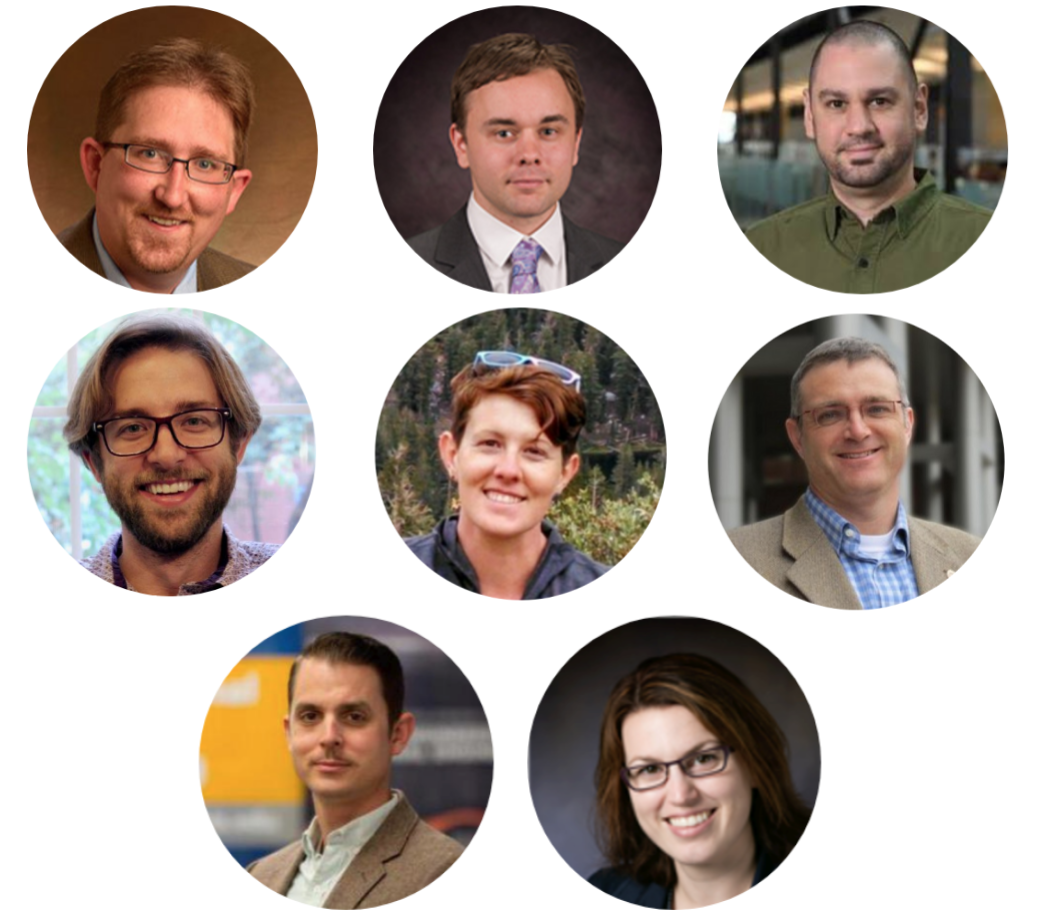
\includegraphics[width=\linewidth]{collaboration-img}\\
                \caption{Nuclear fuel cycle faculty at 6 universities 
                participated. Prof. Neal Davis (Co-PI, CS) and 
                Prof. Jenny Amos (SIIP Liason, BioEng) contributed  
                guidance and perspective within this team.}
	\end{figure}
%\end{block}

%--------------------------------------------------------
% PROJECT TIMELINE
%---------------------------------------------------------
%\begin{block}{Timeline}
        \newcommand\ytl[2]{\parbox[b]{0.3\textwidth}{\hfill{\color{orange!90}\bfseries\sffamily #1}~$\cdots\cdots$~}\makebox[0pt][c]{$\bullet$}\vrule\quad 
\parbox[c]{0.7\textwidth}{\vspace{7pt}\color{dblue!80}\raggedright\sffamily #2\\[7pt]}\\[-3pt]}
\begin{table}
\centering
\begin{minipage}[t]{\linewidth}
\color{gray}
\rule{\linewidth}{1pt}
\ytl{May~2017}{Project start: \hfill GitHub/Video}
\ytl{Jun~2017}{KickOff Workshop\hfill Allerton}
\ytl{Interim}{Remote Collaboration\hfill GitHub/Video}
\ytl{Jun~2018}{Retrospective Workshop \hfill Illini Union}
%\ytl{~~~~~}{~~~~}
%\rule{\linewidth}{1pt}%
%\\%
%\bigskip
%\ytl{~~~~~2019}{Sensitivity analysis: \hfill Vary key parameters.}
\bigskip
\rule{\linewidth}{1pt}%
\end{minipage}%
\end{table}

\end{block}
%----------------------------------------------------------------------------------------
%	BACKGROUND
%----------------------------------------------------------------------------------------
\begin{block}{NECX} 
        The Nuclear Engineering Curriculum eXchange (NECX) is an open 
        repository for nuclear engineering curriculum materials intentionally 
        prepared for \textbf{reuse, remixing and rejeuvination}. We targeted 
        our approach to: 
        \vspace{0.25in}
       
        \begin{itemize}
                \item improve the transfer of lessons learned 
                \item connect instructors of the same course
                \item provide a template for future groups 
                \item scale up for larger courses (e.g. CS101)
        \end{itemize}
%        \vspace{0.25in}
%
%        It relies on:
%
%        \vspace{1cm}
%\begin{itemize}
%        \item lesson component modularity
%        \item well defined learning objectives
%        \item dependency graph of prerequisites
%        \item lesson review by peer faculty
%        \item flexible media and content formats
%\end{itemize}
\end{block}

%----------------------------------------------------------------------------------------
%	NODES
%----------------------------------------------------------------------------------------

\begin{block}{Nodes}
        We identified an \textbf{atomic unit of learning} as
        satisfying at least one learning objective. 

	\begin{figure}
		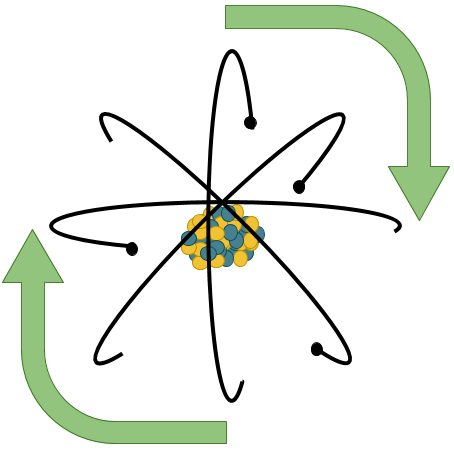
\includegraphics[height=4in]{necx.png}
		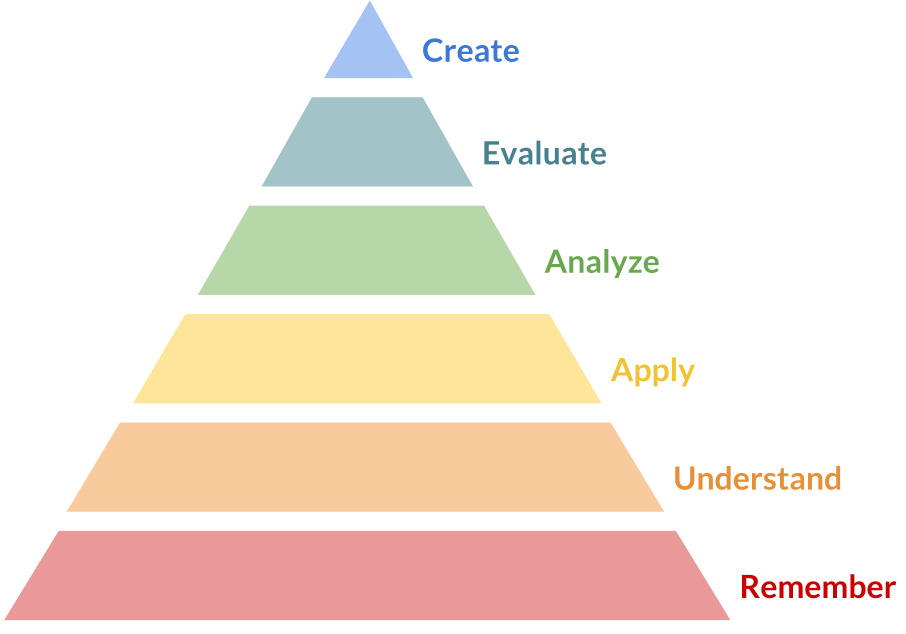
\includegraphics[height=4in]{bloom.png}
	\end{figure}


\end{block}




\end{column} % End of the first column

\begin{column}{\sepwid}\end{column} % Empty spacer column


%----------------------------------------------------------------------------------------

\begin{column}{\onecolwid} % The second column

%----------------------------------------------------------------------------------------
%	Open Source Software Development
%----------------------------------------------------------------------------------------

\begin{block} {Open-Source Software Development}
          \begin{figure}
            \hspace*{-3.5cm}
              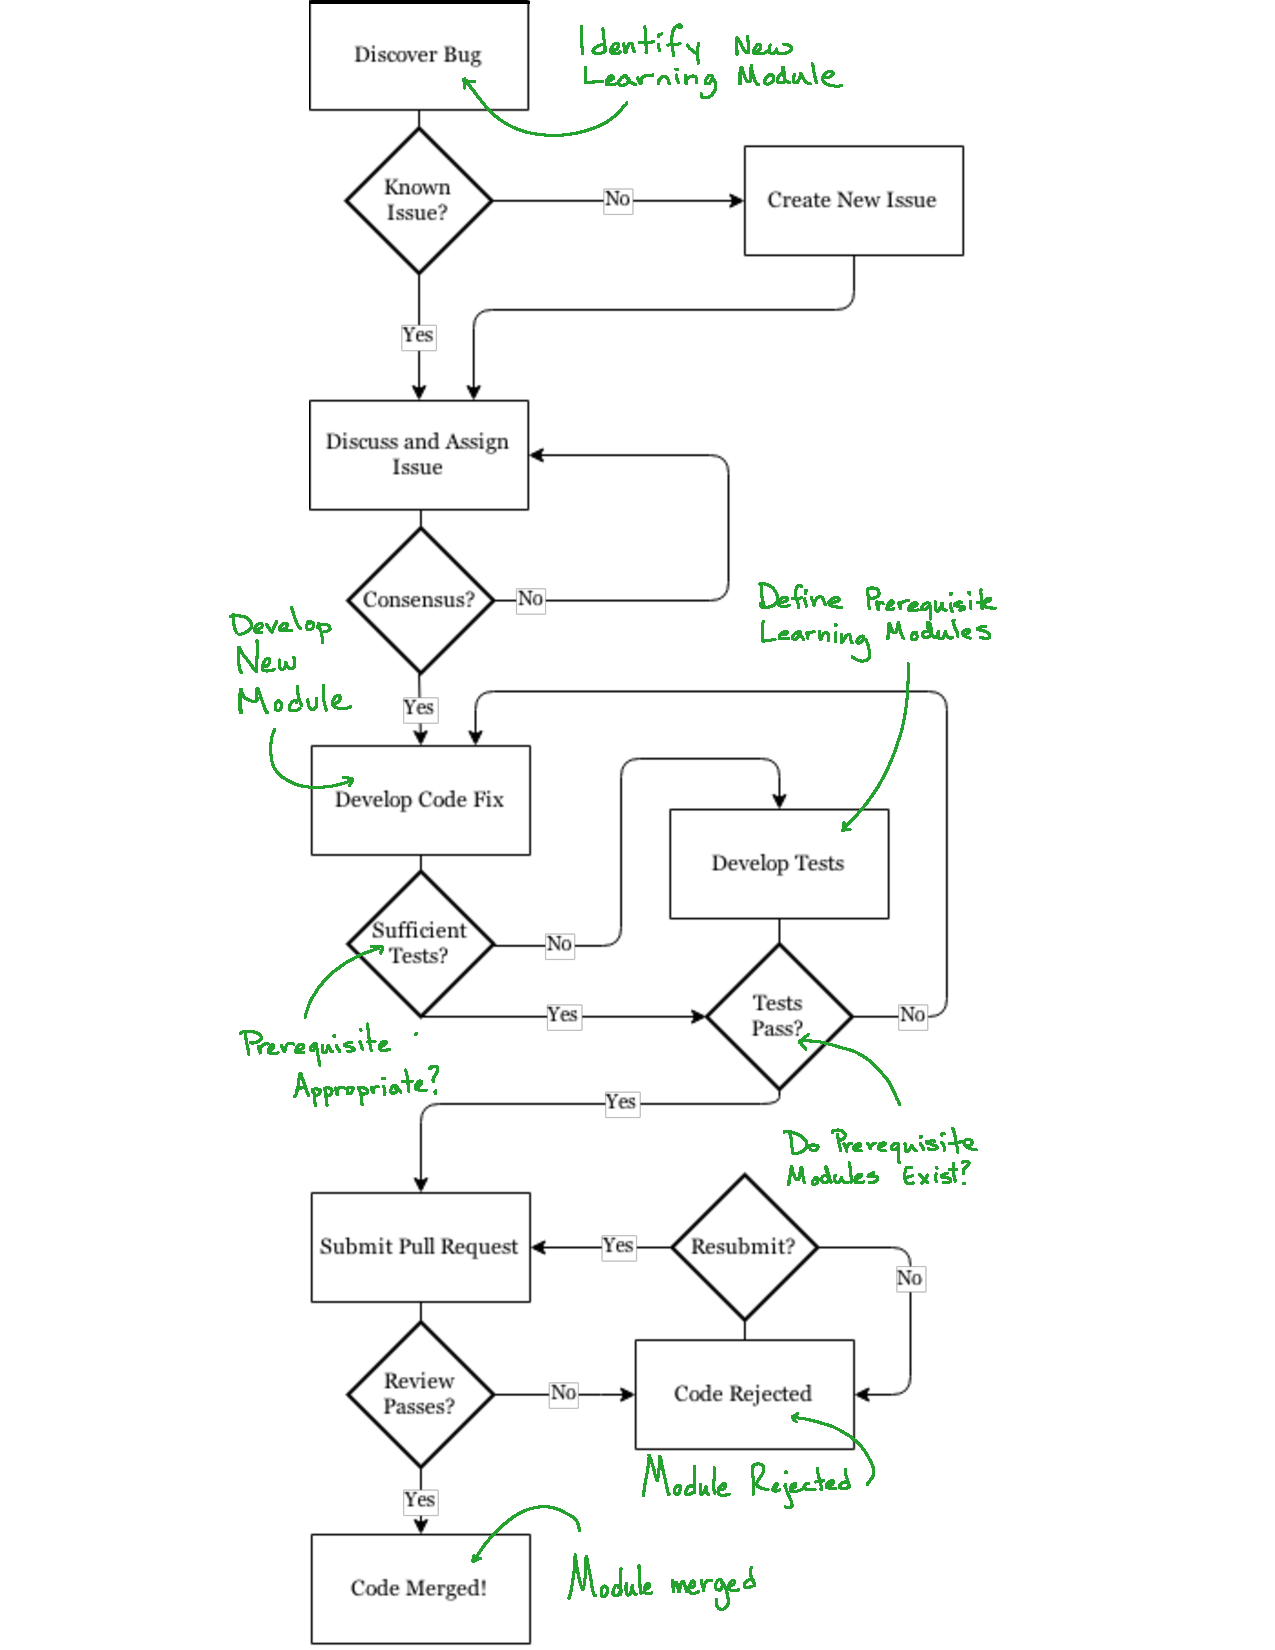
\includegraphics[clip, trim=3cm 0cm 4cm 
                                      0cm, width=1.15\linewidth]{git-flow.pdf}
        \caption{This figure captures the Git Flow process through which a new
                          feature or bug fix enters a piece of open source
                          software. We've adapted this model toward learning 
                          module development on GitHub.}
                                  \label{fig:sub1}
		\end{figure}
                %In a typical open source project, a main copy of the 
                %repository (or main \emph{fork}) holds the official copy of 
                %the software package. Individual developers each have their 
                %own \emph{forks} where they can work on features and bug 
                %fixes. When the developer makes changes that are ready for 
                %prime time, they make a ``pull request'' to the main 
                %\emph{fork}. That \emph{pull request} is reviewed by their 
                %collaborators, and it is eventually merged into the main 
                %\emph{fork} where it can be used by all. Figures 
                %\ref{fig:sub1} and \ref{fig:sub2} show how this open source 
                %software development workflow can be leveraged toward course 
                %development.

\end{block}

\begin{block}{Node Requirements}
        \begin{table}
                \centering
        \begin{tabularx}{\textwidth}{X |X}
                        \hline
                        \textbf{Required} & \textbf{Optional}\\
                        \hline
        \begin{itemize}
        \item a title
        \item a unique short identifying name (UID)
        \item a list of prerequisites based on the UIDs of other nodes
        \item learning objectives
        \item a content summary
        \item at least one assessment object
        \end{itemize} & 
        \begin{itemize}
        \item course notes with equations
        \item example source code
        \item citations of other work
        \item external readings
        \item instructor guidance
        \item graphics
        \item videos
        \item audio files 
        \item worked example problems
        \item ABET Student Outcomes
        \item active learning activities
        \end{itemize}\\
                \end{tabularx}
                \caption{Minimum node requirements and suggested items.}
                \label{tab:node}
        \end{table}

\end{block}

%----------------------------------------------------------------------------------------

\end{column} % End of column 2

\begin{column}{\sepwid}\end{column} % Empty spacer column

\begin{column}{\onecolwid} % The third column
	
%----------------------------------------------------------------------------------------
%	FUTURE WORK
%----------------------------------------------------------------------------------------
\begin{alertblock}{Accomplishments}
	\begin{itemize}
		\item Defined ``Nodes''
		\item Established Contribution Workflow
		\item Created jekyll based website portal
		\item Began Node content creation
	\end{itemize} 
\end{alertblock}


                \centering
		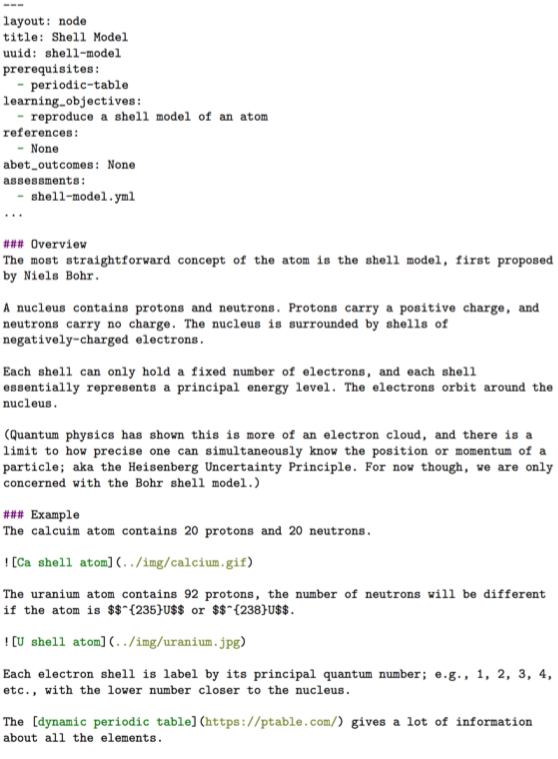
\includegraphics[height=10in]{md-ex.png}

                \vspace{0.5in}
                
\includegraphics[height=1in]{downarrow.png}

                \vspace{0.5in}
		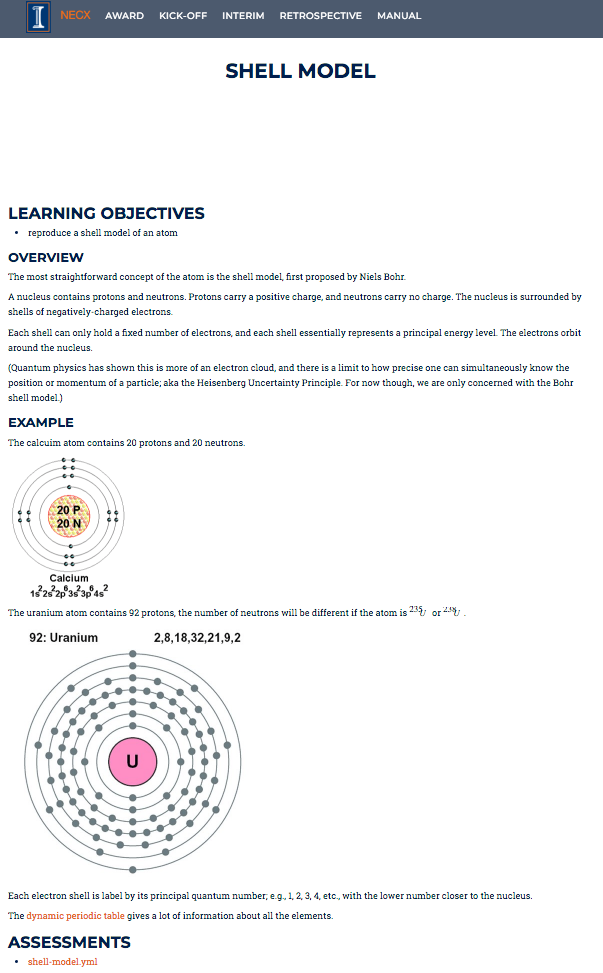
\includegraphics[height=12in]{shell.png}


%----------------------------------------------------------------------------------------
%	ACKNOWLEDGEMENTS
%----------------------------------------------------------------------------------------
\setbeamercolor{block title}{fg=norange,bg=white} % Change the block title color

\begin{block}{Acknowledgements}
	
	This research was performed using funding received
	from the Academy for Excellence in Engineering Education Strategic 
        Instructional Innovation Program (AE3-SIIP) at the University of 
        Illinois. Travel funding was additionally supported by the home 
        institutions of remote participants.
	
%	\vspace{10mm}
%	\begin{center}
%		\begin{tabular}{ccc}
%			
\includegraphics[width=0.3\linewidth]{AE3_logo.png} & \includegraphics[width=0.3\linewidth]{.png}
%			& \includegraphics[width=0.15\linewidth]{cyclus.png}
%		\end{tabular}
%	\end{center}
	
\end{block}


%\begin{block}{References}
%        {\footnotesize\bibliographystyle{abbrv} 
%        \bibliography{poster}}
%\end{block}


%----------------------------------------------------------------------------------------
%	CONTACT INFORMATION
%----------------------------------------------------------------------------------------

\setbeamercolor{block alerted title}{fg=black,bg=norange} % Change the alert block title colors
\setbeamercolor{block alerted body}{fg=black,bg=white} % Change the alert block body colors

\begin{alertblock}{Contact Information}
	\setbeamercolor{block title}{fg=norange,bg=white} % Change the block title color
	\begin{itemize}
		
		\item Web: \href{necx-org.github.io}{necx-org.github.io}
		\item Email: \href{mailto:kdhuff@illinois.edu}{kdhuff@illinois.edu}
	\end{itemize}
	
\end{alertblock}
    

%----------------------------------------------------------------------------------------


\end{column} % End of the third column

\end{columns} % End of all the columns in the poster

\end{frame} % End of the enclosing frame

\end{document}
\begin{column}{\sepwid}\end{column} % Empty spacer column
